\chapter{Software Design}
\label{chap:typeareatest}

Far far away, behind the word mountains, far from the countries Vokalia and Consonantia, there live the blind texts. Separated they live in Bookmarksgrove right at the coast of the Semantics, a large language ocean. A small river named Duden flows by their place and supplies it with the necessary regelialia. It is a paradisematic country, in which roasted parts of sentences fly into your mouth. Even the all-powerful Pointing has no control about the blind texts it is an almost unorthographic life One day however a small line of blind text by the name of Lorem Ipsum decided to leave for the far World of Grammar. 

\section{Software Architecture}
\label{sec:typeareatest_ombox}

The Big Oxmox advised her not to do so, because there were thousands of bad Commas, wild Question Marks and devious Semikoli, but the Little Blind Text didn’t listen. She packed her seven versalia, put her initial into the belt and made herself on the way. When she reached the first hills of the Italic Mountains, she had a last view back on the skyline of her hometown Bookmarksgrove, the headline of Alphabet Village and the subline of her own road, the Line Lane. Pityful a rethoric question ran over her cheek, then she continued her way. On her way she met a copy.

\begin{equation}
	\mathcal{N}(x \mid \mathbold{\mu}, \mathbold{\Sigma}) = \frac{1}{(2\pi)^{D/2}} \frac{1}{|\mathbold{\Sigma}|^{(1/2)}} \exp \left( -\frac{1}{2}(x-\mathbold{\mu})^{T}\mathbold{\Sigma}^{-1}(x-\mathbold{\mu}) \right)
\end{equation}

The copy warned the Little Blind Text, that where it came from it would have been rewritten a thousand times and everything that was left from its origin would be the word "and" and the Little Blind Text should turn around and return to its own, safe country. But nothing the copy said could convince her and so it didn’t take long until a few insidious Copy Writers ambushed her, made her drunk with Longe and Parole and dragged her into their agency, where they abused her for their projects again and again. And if she hasn’t been rewritten, then they are still using her.

\section{Design Decisions}
\label{sec:typeareatest_typedummytext}

This is a typo dummy text. On it you can see if all the letters there are and how they look. Sometimes one uses words like Hamburgefonts, Rafgenduks or Handgloves to test fonts. Sometimes phrases that contain all letters of the alphabet - one calls these sets "pangrams".

Well known is this: The quick brown fox jumps over the lazy old dog. Often in type dummy texts also foreign-language sentence parts are installed (AVAIL\textsuperscript{\texttrademark} and Wefox\textsuperscript{\textregistered} are testing aussi la Kerning) to test the effect in other languages. In Latin, for example, almost every font looks good.

\subsection{Storage Containers}
\label{subsec:satzspiegeltest_typoblindtext_demonstrandum}

Qt has an implementations for all popular storage containers. They all have different structures and are intended for different applications. The Containers can be categorized in two major categories. The first are sequential container each element is stored at a certain index and can be accessed over said index. The second are associative containers and set where all elements are stored with a key. The algorithmic complexity of the  containers are shown in Table ~\ref{tab:qt-container-sequential} for the sequential containers and in Table ~\ref{tab:qt-container-associative}. O(n) stands for linear time so it scales linearly with the size of a container. O(1) stands for constant time, so each operation takes a fixed amount of time no matter how big the container is. O(log(n)) equals linear time. So the cost of an operation on a container raises logarithmic to the number of items in that container. If the behavior is not guarantied it is specified as amortized.

% Please add the following required packages to your document preamble:
% \usepackage{booktabs}
% \usepackage{multirow}

% Please add the following required packages to your document preamble:
% \usepackage{booktabs}
\begin{table}[!htb]
\centering

\begin{tabular}{@{}|l|l|l|l|l|@{}}
\toprule
                                  & Index lookup & Insertion & Prepending  & Appending   \\ \midrule
QLinkedList\textless T\textgreater & O(n)         & O(1)      & O(1)        & O(1)        \\ \midrule
QList\textless T\textgreater       & O(1)         & O(n)      & Amort. O(1) & Amort. O(1) \\ \midrule
QVector\textless T\textgreater     & O(1)         & O(n)      & O(n)        & Amort. O(1) \\ \bottomrule
\end{tabular}
\caption{Algorithmic Complexity of the sequential Qt Containers where each element can be accessed over an index \cite{QtDoc:Containers}}
\label{tab:qt-container-sequential}
\end{table}

\begin{table}[!htb]

\centering
\begin{tabular}{@{}|l|l|l|l|l|@{}}
\toprule

\multirow{2}{*}{}                    & \multicolumn{2}{l|}{Key lookup} & \multicolumn{2}{l|}{Insertion} \\ \cmidrule(l){2-5} 
                                     & Average         & Worst Case    & Average        & Worst case    \\ \midrule
QMap\textless Key, T\textgreater      & O(log n)        & O(log n)      & O(log n)       & O(log n)      \\ \midrule
QMultiMap\textless Key, T\textgreater & O(log n)        & O(log n)      & O(log n)       & O(log n)      \\ \midrule
QHash\textless Key, T\textgreater     & Amort. O(1)     & O(n)          & Amort. O(1)    & O(n)          \\ \midrule
QSet\textless Key\textgreater         & Amort. O(1)     & O(n)          & Amort. O(1)    & O(n)          \\ \bottomrule
\end{tabular}
\caption{Algorithmic Complexity of the associative Qt Containers where each element can be accessed over the associated key \cite{QtDoc:Containers}}
\label{tab:qt-container-associative}
\end{table}

\subsubsection{QLinkedList}
\label{sec:QLikedList}
QLinkedList stores elements by pointing to the previous and next elements, creating a chain that is linked together. Because the pointer to an element is only stored in the adjacent elements, it is slow when accessing an element over an index. However when accessed over an iterator it is possible to insert an element at any point during the traversal of the linked list.

\subsubsection{QList}
\label{sec:QList}
QList allows for fast access over an index and allocates space before and after its internal array which usually results in constant time insertion on both ends of the list as shown in \ref{tab:qt-container-sequential}. It has to be noted that QList allocates its elements on the heap when they use more storage space than a pointer.\cite{QtDoc:QList}
\subsubsection{QVector}
\label{sec:QVector}
QVector is similar to QList as it can also be accessed over an index in constant time. Because QVector doesn't allocate storage before the array it is not possible to prepend objects in constant time. QVector stores each element successively.
\subsubsection{QHash}
\label{sec:QHash}
QHash uses a hash table to store its associated key-value pairs. The advantage of that is fast insertion and lookup of a key, usually in constant time. The hash table is not sorted, so an item with the key ``15'' can be followed by an item with the key ``4''. QHash automaticly grows and shrinks according to the number of stored elements. 
\subsubsection{QMap}
\label{sec:QMap}
QMap is similar in the usage as a QHash. The main difference is that QMap sorts the keys. So an item with the key ``4'' is followed by an item with the key ``15'' when there is no key between the two values. The trade-off for that is slower lookup and insertion of logarithmic time.
\subsubsection{QMultiMap}
\label{sec:QMultiMap}
QMultiMap has the same properties as a QMap but is more convenient if you want to store multiple values per key.
\subsubsection{QSet}
\label{sec:QSet}
QSet is similar to QHash but it does not store a value. An application for a QSet is to store a stream of values without storing duplicates.
\subsection{Containers in Gazelle View}
\label{sec:containersGazelleView}
In Gazelle View there are multiple sets of data that needs to be stored. There are the decoded Frames that need to be handled dynamicaly, the position an the timestamp of each overlay and the timestamp for each frame. Each of those datasets has different requitement and the best storage container needs to be evaluated.
\subsubsection{Framebuffer}
\label{sec:frameBuffer}
Each frame contains a large amount of Data. Around 6 MB per picture for a fullHD stream. Additionally it is also important to store the associated framenumber for each frame. As the buffer is usually a continuous flow of data this can be done with a sequential container with an offset or an associative container with the key represented as frame. Disadvantage of sequential containers are that if you move the first stored frame to the first index the container needs to be rearranged each time frames are deleted. If the frames are stored at the index of their framenumber you have a very large container with mostly empty elements and you need to keep track where how many elements are stored to free the buffer efficiently.

Because the frames don't need to be sorted it is best to use a QHash to store a frame with the framenumber as key. It allows for uncomplicated insertion and checks of how many frames are already stored for handling of the buffersize.
\subsubsection{Overlays}
\label{sec:overlays}
An overlay consists of the position where it should be placed and the timestamp when it should be displayed. Access is usually over a timestamp to get an overlay that is before or after said timestamp. To accomplish that the container needs to be associative and sorted. QMap fulfills those requirements perfectly.
\subsubsection{Timestamps}
\label{sec:timestamps}
The timestamps consists out of a continuous list of timestamps for each frame. It needs to be possible to access the timestamp for each frame and the frame before a timestamp. There are a few options to solve this dual access problem. 

The first is a QVector where each timestamp is stored at the index of the corresponding frame. The advantage of that approach is that it is not memory intensive and access of a timestamp of a frame is done in constant time. But o get the frame for a timestamp requires iterating over the QVector resulting in linear time access. As there may be multiple of 10'000 frames per video this is not desirable. 

Another option would consist of a QVector for the timestamps and a QMap for accessing the framenumber from a timestamp. The access over a QMap reduced the time needed from linear to logarithmic time for the cost of duplicating the stored information. 

A third option exploits the fact that timestamps count up. So it is possible to get the correct frame out of timestamps stored in a QVector in logarithmic time with the usage of successive approximation to calculate the frame. As this combines the small memory footprint as the first and fast access of the second option it is the best choice for this problem.


\section{Webstandards}+
\label{sec:satzspiegeltest_webstandards}

Everywhere the same old story. The layout is complete, the text is slow in coming. This layout is now not naked in space and small and empty occurs, I help out: the dummy text. Created exactly for this purpose, always in the shadow of my big brother "Lorem Ipsum", I look forward every time you read a few lines. Because esse est percipi - being is to be perceived.

And now because you already have the goodness to accompany me a few more sentences long, I would like to take this opportunity to serve you not only as a stopgap, but to point out something that is going to be perceived as deserved: Web viz. See Web standards are the rules that build on the websites. So there are rules for HTML, CSS, JavaScript or XML, words that you might have heard of your developers. These standards ensure that all parties the maximum benefit from a website.

\begin{figure}[H]
	\centering
		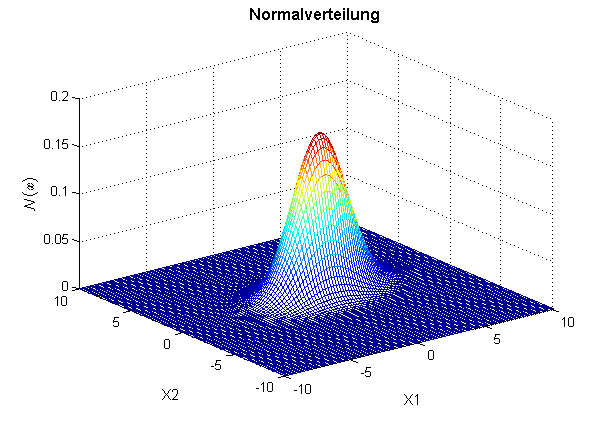
\includegraphics[scale=0.7]{images/multivariate_gauss.png}
	\caption{Normal distribution}
	\label{fig:normal_distribution}
\end{figure}

In contrast to previous websites we no longer need, for example, two different sites for the program Internet Explorer and another browser. It extends a page that - properly applied - both works on different browsers on the net, but just as good for printing or display on a cell phone is. Mind: A site for all formats. What a relief. Standards save time provide for the development costs and ensure that web pages can be easier to maintain later. Of course, only if everyone adheres to these standards.
